% !TEX program = xelatex

% “..”表示返回上一级目录，LaTeX 会自动补上 .cls
\documentclass[withoutpreface,bwprint]{../cumcmthesis}

% 从 primary template.tex 复制需要的宏定义
\newcommand{\RR}{\mathbb{R}}
\newcommand{\argvec}{\arg}
\newcommand{\diam}{\operatorname{diam}}
\newcommand{\wrap}{\operatorname{wrap}}
\newcommand{\MEC}{\operatorname{MEC}}

\begin{document}

\section{问题三、问题四预览}

% 载入同一文件夹中的论文初稿
% 问题三、问题四正文初稿（可迁移片段）
% 说明：本文件不含 \documentclass、宏包和 document 环境。
% “问题分析”块分别替换 primary template.tex 中的问题3分析、问题4分析；
% “模型建立与求解”块替换原有问题3、问题4占位内容。
% 仅使用 cumcmthesis.cls 已加载的环境和 primary template.tex 已定义的记号。
% 当前算法口径：problem3_solver_shared.m 与 problem4_solver_split.m。

% =====================================================================
% 第一部分：放入 \section{问题分析}
% =====================================================================

\subsection{问题3分析}

问题三要求机器狗在干扰源数量、频道和位置均未知的条件下，完成对全向干扰源的搜索、
定位与清除。任务中的移动、频道切换、无线电检测和光学清除共同增加时长。

因此该问题不是单纯的定位问题，而是连续区域覆盖、带误差定位和动态路径规划的耦合问题。

为确保所有干扰源均被发现，首先依据最小有效接收半径设计覆盖整个目标圆域的检测点
设计方案，其基本思想如图~\ref{fig:p3-cover-scheme} 所示。

在发现干扰源后，沿用问题一的
交会定位区域和问题二的最小包围圆，持续更新各频道的位置可行域。

考虑到机器狗移动耗时在总时间中占比较高，
不能将搜索和清除分成两个彼此独立的阶段，否则会造成重复路程；因此，将尚未访问的
必要搜索站与已发现但尚未清除目标的包围圆圆心放入同一条动态开放路径中统一排序,实现搜索与清除的同步进行。

在此基础上，局部定位点不只服务于当前目标。当该点对其他已发现且定位误差仍较大的
频道同时满足接收距离保证和几何收益判据时，机器狗在同一位置追加这些频道的测向，
以共享已经发生的移动成本。若没有频道通过筛选，则仍只检测当前目标，不改变原有定位流程。

模拟器只返回 \texttt{no\_signal}、\texttt{near} 或 \texttt{direction}，并不返回
数值场强；且同一地点的测向误差保持不变。因此，本文不利用场强反演距离，也不通过
同点重复测量降低误差，而是利用不同位置形成的测向误差带交会来缩小可行域，但实际应用中可以考虑这些因素进一步优化算法，减少总时间。

\begin{figure}[htbp]
\centering
\IfFileExists{问题3，4论文及可视化/图_问题三检测点覆盖方案.pdf}
{
\includegraphics[width=0.96\textwidth]{问题3，4论文及可视化/图_问题三检测点覆盖方案.pdf}}
{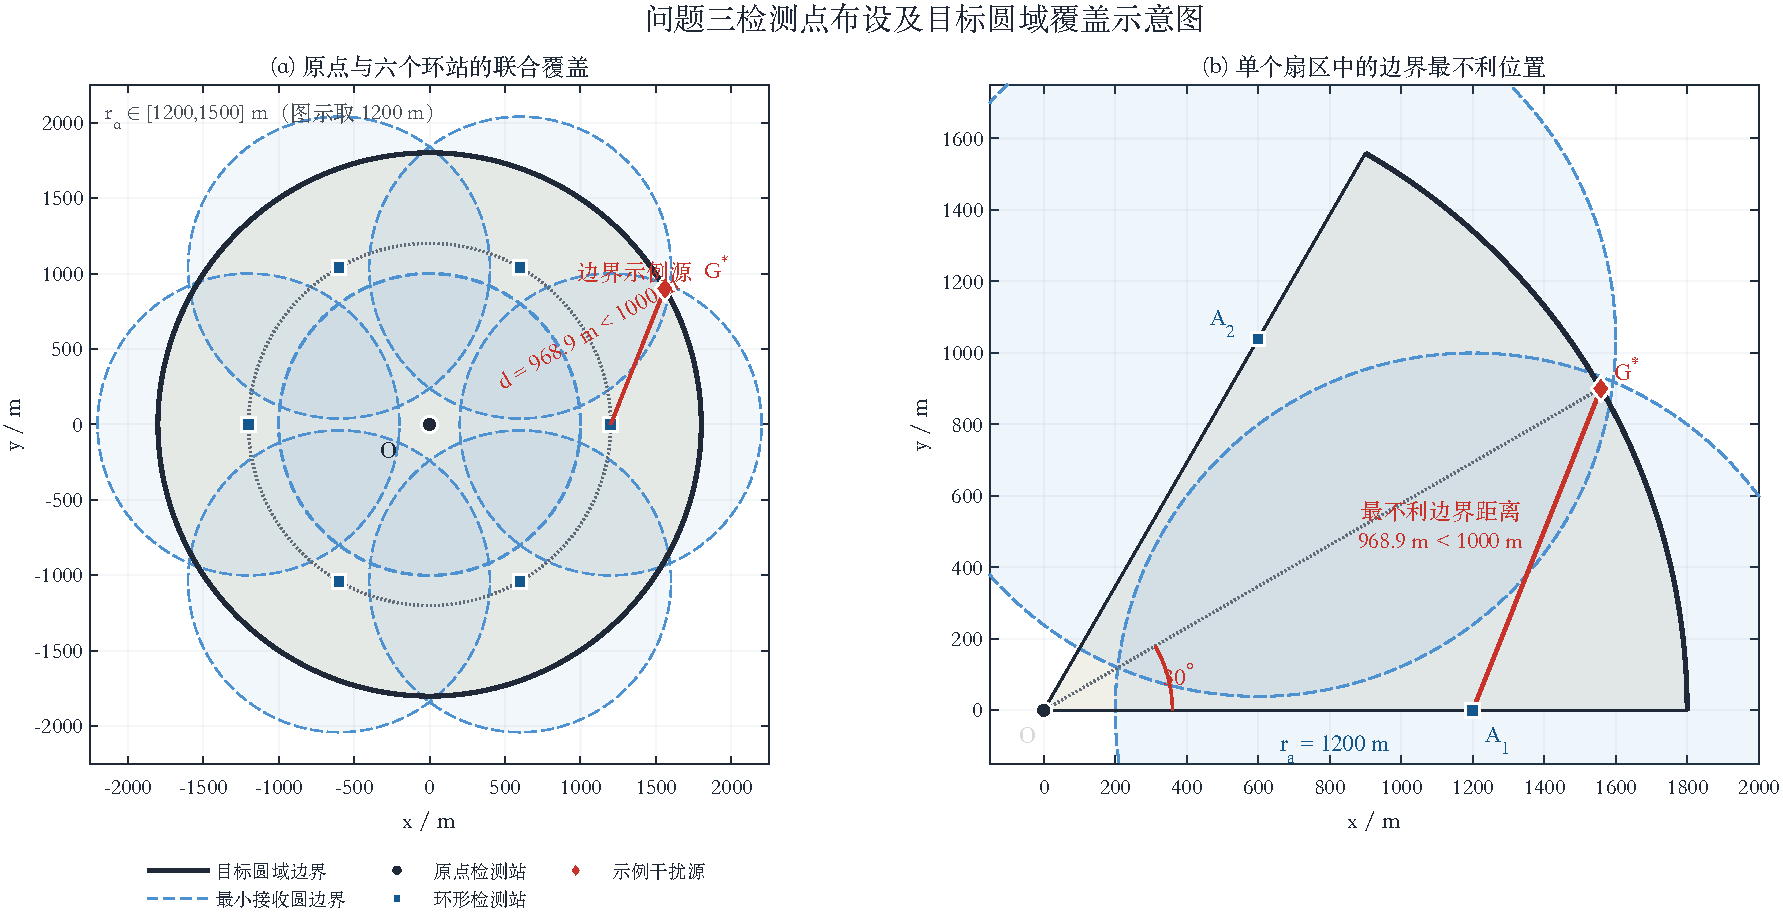
\includegraphics[width=0.96\textwidth]{图_问题三检测点覆盖方案.pdf}}
\caption{问题三自适应六边形检测点布设与边界最不利位置}
\label{fig:p3-cover-scheme}
\end{figure}


\subsection{问题4分析}

问题四同时存在全向与定向干扰源。定向源只在某个闭半平面内辐射信号，故单点的
\texttt{no\_signal} 可能由频道为空、距离过远或检测点位于定向覆盖范围外三种原因造成，
不能据此直接排除某一区域。搜索阶段需要构造对任意发射半平面均有效的确定性站点覆盖；
定位阶段则需要在全向源的快速交会方法和定向源的稳健追踪方法之间进行分流。

本文先保留“全向源”这一工作假设。当某个检测点对当前整个位置可行域均满足接收距离
保证，而该点仍无信号时，才能排除距离因素并严格确认该源为定向源。这样既能让信号
稳定的干扰源沿用问题三的可行域更新与中心清除方法，又不会利用未经证明的频道淘汰
牺牲全清率。

% =====================================================================
% 第二部分：放入 \section{模型的建立与求解}
% =====================================================================

\subsection{问题3：全向干扰源的动态搜索、定位与清除}

\subsubsection{时间目标与频道状态}

设机器狗依次执行的动作位置为 $X_0,X_1,\ldots,X_M$，其中 $X_0=(0,0)$。
记总移动距离为
\begin{equation}
L=\sum_{j=1}^{M}\|X_j-X_{j-1}\|,
\end{equation}
检测次数、频道切换次数、光学探测次数和成功清除次数分别为
$N_{\mathrm m},N_{\mathrm s},N_{\mathrm o},N_{\mathrm c}$。根据附件给出的计时规则，
一次成功清除包含 $3$ 秒光学探测和 $2$ 秒激光清除，因此总虚拟时间为
\begin{equation}
T=\frac{L}{5}+N_{\mathrm s}+5N_{\mathrm m}+3N_{\mathrm o}+2N_{\mathrm c}.
\label{eq:p3-time}
\end{equation}
设真实干扰源总数为 $N$，被清除数量为 $C$。问题三可写成带硬约束的优化问题
\begin{equation}
\min T,\qquad \text{s.t.}\quad C=N,
\label{eq:p3-objective}
\end{equation}
并以清除比例 $C/N$ 和平均定位清除时间 $T/C$ 评价算法。

对每个频道 $k\in\{1,\ldots,20\}$，在线维护“未发现”“已发现待定位”和“已清除”
三类状态。已发现频道还维护位置可行多边形 $\Omega_k$、其最小包围圆圆心 $c_k$ 与半径
$r_k$。

为便于后续利用半平面交连续裁剪可行域，并使 \(\Omega_k\) 始终保持为凸多边形，本文以目标圆域的外切正 \(64\) 边形初始化 \(\Omega_k\)。该外近似完整包含真实圆域，不会因离散化排除真实位置；其最大径向外扩仅为  
\[
1800\left[\sec\left(\frac{\pi}{64}\right)-1\right]\approx2.17\ \mathrm m,
\]因而能够兼顾算法的保守性与计算效率。

若在位置 $q$ 得到示向度
$\theta$，则利用问题一的楔形半平面算法进行更新：
\begin{equation}
\Omega_k\leftarrow
\Omega_k\cap W(q,\theta,1.005^\circ)
\cap\left\{x:u(\theta)^{\mathsf T}(x-q)\le 1500\right\},
\label{eq:p3-region-update}
\end{equation}
其中 $u(\theta)=(\cos\theta,\sin\theta)^{\mathsf T}$。将误差界从 $1^\circ$
略放宽为 $1.005^\circ$，用于容纳接口将示向度保留两位小数产生的舍入误差。
更新后调用问题一的直径算法和问题二的最小包围圆算法计算 $(c_k,r_k)$。

\subsubsection{连续圆域的覆盖方案}

记目标区域为
\begin{equation}
\mathcal D=\left\{x\in\RR^2:\|x\|\le1800\right\}.
\end{equation}

由于问题三中的干扰源均为全向源，且有效接收半径不小于 \(1000\ \mathrm m\)，机器狗在位置 \(q\) 扫描全部未知频道后，可排除圆盘 \(B(q,1000)\) 内存在尚未发现干扰源的可能。因此，完成全局排查等价于验证历次扫描圆盘的并集是否覆盖整个连续区域 \(\mathcal D\)。直接动态维护多个圆盘的并集及其未覆盖曲边区域较为繁琐，故本文用边长 \(h=20\ \mathrm m\) 的正方形网格覆盖 \(\mathcal D\)，以有限个尚未被安全覆盖的网格单元记录剩余待排查区域。且使用网格的中心点\(g\)的扫描状态代表整个网格的扫描状态，则单元内任一点到 \(g\) 的距离均不超过其外接半径
\[
\delta=\frac{h}{\sqrt2}=14.142\ \mathrm m.
\]因此，当且仅当扫描点 \(q\) 满足
\[
\|g-q\|\le R_{\mathrm{cov}}
\equiv1000-\delta-\varepsilon
\]时，对单元内任意一点 \(x\)，由三角不等式有
\[
\|x-q\|
\le\|x-g\|+\|g-q\|
\le\delta+1000-\delta-\varepsilon
<1000,
\]从而保证整个网格单元均处于无线电扫描的可靠覆盖范围内。

为构造具有确定覆盖保证的搜索方案，首先考虑由原点与正六边形六个顶点组成的七点扫描骨架。设正六边形的外接圆半径为 $r_a$，六个环形扫描站为
\begin{equation}
A_j=r_a
\left(
\cos\frac{j\pi}{3},
\sin\frac{j\pi}{3}
\right)^{\mathsf T},
\qquad j=0,1,\ldots,5.
\end{equation}

下面说明，当
\begin{equation}
1200\le r_a\le1500
\end{equation}
时，原点与六个环形扫描站均能完成对目标圆域的连续覆盖。

考虑任一与目标圆域 $\mathcal D$ 相交、但未被原点覆盖的网格单元，记其中心为 $g$，并令 $\rho=\|g\|$。由网格构造可知
\begin{equation}
R_{\mathrm{cov}}<\rho\le1800+\delta.
\end{equation}
在六个环形扫描站中，取极角与 $g$ 最接近的点 $A_j$，则二者的极角之差不超过 $30^\circ$。由余弦定理，
\begin{equation}
\|g-A_j\|^2
\le
\rho^2+r_a^2-2\rho r_a\cos30^\circ.
\end{equation}
对
\[
\rho\in[R_{\mathrm{cov}},\,1800+\delta],
\qquad
r_a\in[1200,\,1500]
\]
的端点组合进行检验可知，最不利情形为
$\rho=1800+\delta$、$r_a=1200$，此时
\begin{equation}
\|g-A_j\|<980.05\ \mathrm m
<R_{\mathrm{cov}}\approx985.86\ \mathrm m.
\end{equation}
因此，任取 $r_a\in[1200,1500]$，原点与六个环形扫描站均能覆盖全部网格单元，从而保证目标圆域内的干扰源不会因搜索盲区而遗漏。

据此，基础算法固定取
\begin{equation}
r_a=1500\ \mathrm m,
\end{equation}
形成一组预先确定的七点搜索骨架。机器狗依次完成这些位置的必要频道扫描，即可实现对整个目标圆域的可靠排查；再结合后续的定位与清除步骤，便可完成问题三的基本任务。

固定半径方案虽然具有确定的覆盖保证，但没有利用原点扫描获得的场景信息。当原点扫描后已经发现较多频道时，通常意味着需要依靠外围搜索发现的剩余频道较少，此时仍访问半径为 $1500\ \mathrm m$ 的环形站点可能产生不必要的移动；反之，当原点发现的频道较少时，应保留较大的搜索半径，以加强对外围区域的排查。因此，在基础方案上引入基于初始观测的自适应选径：
\begin{equation}
r_a=\max\{1200,\ 1500-60n_0\},
\label{eq:p3-anchor-radius}
\end{equation}
其中 $n_0$ 为原点首次扫描发现的频道数。该规则使环形骨架随 $n_0$ 增大而向内收缩，同时始终保证
$r_a\in[1200,1500]$，因而只改变搜索效率，不影响前述连续覆盖保证。

系数 $60$ 和下界 $1200\ \mathrm m$ 属于效率参数，而非覆盖成立的必要条件。后文将在相同随机场景下分别运行固定半径方案与自适应方案，通过配对蒙特卡洛模拟比较二者的移动距离和总耗时，以检验自适应骨架的实际优化效果。

固定环站到达后必定检测所有仍有必要检测的频道，并删除其覆盖的网格。局部定位或清除
产生的停留点也可以参与区域排查：一个全局任务结束后，若当前位置新增覆盖面积达到
$0.8\ \mathrm{km}^2$，或当前没有待处理目标，则在该处检测全部未知频道以及满足
$r_k>60$ m 的已知未清除频道，再删除相应网格。该门槛用于避免在相邻局部点频繁空扫。

\subsubsection{搜索站与待处理干扰源的动态开放路径}

设当前机器狗位置为 $p$，已检测到的尚未清除干扰源的包围圆圆心集合为 $\mathcal C$，
仍能覆盖未排查网格的环站集合为 $\mathcal A$。把两类任务合并为
\begin{equation}
\mathcal V=\mathcal C\cup\mathcal A.
\end{equation}
将访问次序记为双射
\begin{equation}
\pi:\{1,2,\ldots,|\mathcal V|\}\longrightarrow\mathcal V,
\end{equation}
其中 $\pi(j)$ 表示第 $j$ 个访问的任务点。相应的开放路径长度为
\begin{equation}
L(\pi)=\|p-\pi(1)\|+
\sum_{j=1}^{|\mathcal V|-1}\|\pi(j+1)-\pi(j)\|.
\label{eq:p3-open-route}
\end{equation}
由于任务集合 $\mathcal V$ 会随观测结果变化，算法不求解一次性的闭合旅行商回路。
每次全局规划先采用最近邻贪心策略构造初始开放路径，即依次选择距离当前位置最近的
未访问任务点；随后采用 2-opt 局部搜索，通过反转部分访问次序消除路径交叉和不必要
折返。算法只选取该路径的首个任务：若其为环站，完成必要频道扫描后返回全局层；若其为
目标圆心，则进入该频道的局部定位子过程，完成清除或执行光学兜底后再返回全局层。
此后从机器狗的新位置更新 $\mathcal C$、$\mathcal A$ 并重新规划。已经被顺路扫描覆盖的
环站会因不再覆盖未排查网格而自动退出任务集合。

在环站或触发区域排查的停留点上，算法优先检测测向机当前频道，再按编号检测其余必要
频道，以减少频道切换；在局部定位点上，则先检测当前目标频道，再考虑共享检测。

\subsubsection{局部点的同点多频道共享观测}

设机器狗为频道 $k$ 选定局部检测点 $q$。算法先检测频道 $k$，再从其他已发现、未清除且
$r_\ell>60$ m 的频道中筛选可共享频道。首先要求
\begin{equation}
d_{\max,\ell}(q)=\max_{x\in\Omega_\ell}\|x-q\|\le1000,
\label{eq:p3-share-safe}
\end{equation}
并要求 $q$ 不与频道 $\ell$ 的上一次测向位置重合。式~\eqref{eq:p3-share-safe} 保证无论
真实源位于当前可行域何处，该点均在最小有效接收半径内，因此共享检测不会出现由距离
过远造成的无信号。

为避免增加收益很小的测量，进一步设置几何收益筛选。记 $a_\ell$ 为 $\Omega_\ell$ 顶点
中心化后第一主轴的单位方向，$b_\ell=c_\ell-q$，要求
\begin{equation}
\|b_\ell\|\ge\max\{100,0.4r_\ell\},\qquad
\frac{|a_{\ell,1}b_{\ell,2}-a_{\ell,2}b_{\ell,1}|}{\|b_\ell\|}
\ge\sin30^\circ.
\label{eq:p3-share-geometry}
\end{equation}
前一条件保证观测基线足够长，后一条件要求新示向线与当前可行域长轴充分交叉。最后，
从可行域边界均匀选取至多 $8$ 个代表点并加入圆心，对每个代表位置分别代入
$-1^\circ,0,1^\circ$ 三种测向误差；仅当所有试算所得最小包围圆半径均不超过 $60$ m
时，才实际检测频道 $\ell$。该预测只用于决定是否共享，不计入虚拟时间。安全性由
式~\eqref{eq:p3-share-safe} 保证，式~\eqref{eq:p3-share-geometry} 与有限样本试算则用于
控制效率；即使没有其他频道通过筛选，当前目标频道的定位与全局覆盖仍照常进行。

\subsubsection{自适应交会与光学兜底}

对待定位频道 $k$，根据当前最小包围圆半径 $r_k$ 选择动作：
\begin{enumerate}
    \item 当 $r_k\le60$ m 时，先在 $c_k$ 尝试光学清除。若未成功，则机器狗已经位于
    $c_k$，立即原地测向并继续收缩 $\Omega_k$。
    \item 当 $r_k>60$ m 时，令 $e=(c_k-p)/\|c_k-p\|$，在圆心附近选取
    \begin{equation}
    q=c_k+\min\{80,r_k/2\}
    \begin{pmatrix}-e_2\\e_1\end{pmatrix},
    \label{eq:p3-side-step}
    \end{equation}
    作为下一检测点。该侧向位移可避免新旧示向线近似共线。
    \item 对同一目标最多执行 $12$ 轮上述局部交会；若仍未完成清除，则在
    $\Omega_k$ 的外接矩形上采用间距 $25$ m 的
    蛇形光学扫描。网格覆盖半径为 $25/\sqrt2=17.68$ m，小于光学清除半径 $20$ m，
    因而该步骤能够作为数值退化情形下的确定性兜底。
\end{enumerate}
每个局部点均先检测目标频道，再按上一节的条件复用该位置检测其他粗定位频道。若任一
检测结果为 \texttt{near}，则相应干扰源距离机器狗不超过 $5$ m，算法直接调用光学清除。

% [VIS-P3-2] 此处可选插入“同一种子下原优化款与共享观测款的轨迹及共享测量点对照”。

综合以上步骤，问题三算法如下：
\begin{enumerate}
    \item 在原点按当前频道优先顺序扫描全部 $20$ 个频道，建立初始可行域；
    \item 根据原点发现数确定六边形半径，并建立未排查网格集合；
    \item 合并待处理目标圆心与仍有覆盖贡献的环站，采用最近邻贪心和 $2$-opt 生成
    动态开放路径，并选取首个全局任务；
    \item 若该任务为环站，则检测全部未知频道以及 $r_k>60$ m 的已知未清除频道，并
    更新未排查网格；若为目标，则进入至多 $12$ 轮的中心清除或侧向交会，并在每个
    局部点筛选可共享频道，必要时执行光学兜底；
    \item 一个全局任务完成后更新频道状态、可行域和任务集合，并从当前位置重新规划；
    直至已清除 $16$ 个干扰源，或连续圆域已全部排查且所有已发现频道均被清除，最后
    调用 \texttt{/exit}。
\end{enumerate}

由式~\eqref{eq:p3-cell-cover} 及七点骨架的覆盖性，未排查集合为空意味着每个可能的
全向干扰源均曾处于一次对应频道的有效接收范围内，故不存在未发现干扰源。另一方面，
每次测向更新均保留真实位置；共享检测只在式~\eqref{eq:p3-share-safe} 成立时加入新的
有效约束，不会破坏这一性质；光学兜底又覆盖整个可行域。因此，在题设误差和接口规则下，
算法的搜索与清除两部分均保留确定性覆盖保证。

\subsubsection{蒙特卡洛演练与分层比较}

为在正式测试前检验算法，构造与附件计时和反馈规则一致的封闭模拟器。每个案例随机生成
$10\sim16$ 个互异频道；均匀场景中的位置按面积均匀分布，有效接收半径在
$[1000,1500]$ m 上均匀生成。配对算法共享源数、频道、位置、接收半径及
“位置--频道”固定误差场，且只能读取接口反馈，不能访问场景真值。

首先检验覆盖与路径层的改进。基础款使用固定半径 $1500$ m 的六边形和较粗覆盖网格；
骨架优化款采用式~\eqref{eq:p3-anchor-radius} 的自适应骨架与 $20$ m 网格。配对结果见
表~\ref{tab:p3-mc}。

\begin{table}[htbp]
\centering
\small
\caption{问题三基础款与骨架优化款的配对蒙特卡洛结果}
\label{tab:p3-mc}
\begin{tabular}{lrrrrrr}
\toprule
场景 & 配对数 & 基础款/(s/源) & 骨架优化/(s/源) & 节省/(s/源) & 优化比例 & 全清率 \\
\midrule
均匀分布 & 200 & 300.03 & 275.98 & 24.05 & 8.02\% & 100\% \\
边界源   & 80  & 323.36 & 323.60 & $-0.24$ & $-0.07\%$ & 100\% \\
极限条件 & 80  & 304.67 & 290.75 & 13.92 & 4.57\% & 100\% \\
\bottomrule
\end{tabular}
\end{table}

均匀场景下，骨架优化款在 $87.5\%$ 的配对案例中更快，每源平均节省的 $95\%$ 近似置信区间为
$[21.02,27.08]$ s；平均时间低于 $300$ s 的案例比例由 $54.5\%$ 提高到 $71.0\%$。
总时间的下降主要来自移动时间由每场 $2788.40$ s 降至 $2542.79$ s。边界压力场景下
两算法近似持平，说明自适应内缩对一般场景有效，但没有改善所有干扰源均位于最外边界时的
路线。三类测试共 $360$ 个配对案例，两算法均完成全部清除且未出现接口模拟错误。

最终算法在骨架优化款上继续加入同点多频道共享观测。对该层仍采用相同的配对框架比较
“骨架优化款”和“共享观测款”，并额外统计每场共享测量次数、共享停留点数及其对移动
时间和检测时间的净影响，以判断共享移动成本能否抵消新增频道检测的时间。

% TODO-P3-SHARED-MC：现有共享版结果早于本次代码恢复；冻结当前程序后重新运行并补入数值。

% [VIS-P3-3] 此处建议插入“共享观测前后的配对差值、共享次数与耗时分解”。

\subsubsection{问题三正式测试结果}

表~\ref{tab:p3-official} 按题目要求预留三次正式测试记录。案例编码、清除数量和时间必须
在正式测试及日志导出完成后据实填写，不能以蒙特卡洛结果代替。

\begin{table}[htbp]
\centering
\caption{问题三正式测试结果（待正式测试后填写）}
\label{tab:p3-official}
\begin{tabular}{ccccc}
\toprule
测试 & 案例编码 & 清除干扰源个数 & 平均定位清除时间/s & 程序运行时间/s \\
\midrule
测试1 & -- & -- & -- & -- \\
测试2 & -- & -- & -- & -- \\
测试3 & -- & -- & -- & -- \\
\bottomrule
\end{tabular}
\end{table}

\subsection{问题4：混合方向干扰源的确定性覆盖与分流追踪}

\subsubsection{双环站点的全方向覆盖}

问题四中定向源的辐射区域是以干扰源为边界点的一个闭半平面。仅使用问题三的七点骨架，
不能保证任意定向半平面内都存在距离不超过 $1000$ m 的检测点。为此构造如下 $25$ 个
全局搜索站：
\begin{equation}
\begin{aligned}
S_0&=(0,0)^{\mathsf T},\\
S_j^{\mathrm{in}}&=950
\left(\cos\frac{j\pi}{6},\sin\frac{j\pi}{6}\right)^{\mathsf T},\\
S_j^{\mathrm{out}}&=1865
\left(\cos\left(\frac{j\pi}{6}+\frac{\pi}{12}\right),
\sin\left(\frac{j\pi}{6}+\frac{\pi}{12}\right)\right)^{\mathsf T},
\end{aligned}
\qquad j=0,1,\ldots,11.
\label{eq:p4-stations}
\end{equation}

外环正十二边形的内切圆半径为
$1865\cos15^\circ=1801.45$ m，大于目标圆半径，故目标圆包含在此外环多边形内。
连接原点、内环与错开 $15^\circ$ 的外环进行三角剖分，三类可能的较长边分别为
\begin{equation}
\begin{aligned}
d_1&=950,\\
d_2&=2\times1865\sin15^\circ=965.40,\\
d_3&=\sqrt{950^2+1865^2-2\times950\times1865\cos15^\circ}=978.76.
\end{aligned}
\end{equation}
均小于最小接收半径 $1000$ m。因此，任一干扰源 $G$ 所在的小三角形的三个顶点到
$G$ 的距离均不超过 $1000$ m。

任意一条经过 $G$ 的直线都不可能把上述三角形的三个顶点全部严格分隔到不含该三角形
内部的同一侧；故定向源的任一闭发射半平面中至少包含一个三角形顶点。该顶点同时满足
距离约束和角度约束，从而必能接收到信号。式~\eqref{eq:p4-stations} 因此给出了兼容全向
与任意定向方向的确定性发现保证。

% [VIS-P4-1] 此处建议插入“25点双环三角剖分与定向半平面覆盖证明”。

全局阶段把未访问站点与待处理源的可行域圆心合并，仍采用最近邻和 $2$-opt 求动态开放
路径。每到一个全局站，对所有未发现频道进行检测；已发现但尚未清除的频道最多顺路积累
六条示向线。若已清除 $16$ 个源，则由数量上界可直接结束；否则须完成全部 $25$ 点排查并
清除所有已发现源。

\subsubsection{定向源的成对前探与窄带光学覆盖}

设某频道最近一次有效检测点为 $q_0$，示向度为 $\theta$，记
\begin{equation}
u=(\cos\theta,\sin\theta)^{\mathsf T},\qquad
v=(-\sin\theta,\cos\theta)^{\mathsf T},
\end{equation}
并令
\begin{equation}
U=\min\left\{1500,\ \max_{x\in\Omega_k}\|x-q_0\|\right\}.
\end{equation}
当 $U\le600$ m 时，测向误差带在最远处的半宽为
\begin{equation}
w=U\sin1.005^\circ\le10.52\ \mathrm m<20\ \mathrm m.
\end{equation}
沿中心示向线按
\begin{equation}
\Delta x=1.98\sqrt{20^2-w^2}
\label{eq:p4-ray-step}
\end{equation}
布置光学清除点，相邻半径 $20$ m 的清除圆即可覆盖整条测向窄带。

当 $U>600$ m 时，令
\begin{equation}
a=\min\{490,0.6U\},\qquad b=a\tan1.005^\circ+3,
\end{equation}
并在测向线两侧构造一对检测点
\begin{equation}
Q_\pm=q_0+au\pm bv.
\label{eq:p4-paired-probes}
\end{equation}
侧移量 $b$ 严格大于误差楔在推进截面上的半宽。若干扰源尚在该截面前方，则真实射线
与线段 $Q_-Q_+$ 相交。记真实方向与 $u$ 的夹角为 $\varphi$，由
$|\varphi|\le1.005^\circ$、$a\le490$ m 以及干扰源位于截面前方，可验证
$\|Q_\pm-G\|\le\|q_0-G\|$，故两个探测点均不超出 $q_0$ 所对应的有效接收半径。
又因为 $q_0$ 曾接收到信号，定向发射半平面至少覆盖 $Q_-$、$Q_+$ 中的一点。
算法优先访问离当前位置较近的探测点，必要时再访问另一点。
若两点均无信号，则干扰源必位于推进截面之前，转而对长度
$a/\cos1.005^\circ+1$ 的窄带执行式~\eqref{eq:p4-ray-step} 的光学覆盖。

经过最多五轮成对前探仍未清除时，使用第一次有效示向度建立最终兜底。由最大接收距离
可知真源位于长度 $1500$ m、最远半宽
$1500\sin1.005^\circ=26.31$ m 的条带内。沿纵向以 $28$ m 为间距，并在横向
$-42,-14,14,42$ m 四条线上作蛇形扫描，任一点到最近扫描点的距离不超过
$\sqrt{14^2+14^2}=19.80$ m，因此必能进入光学清除范围。该兜底仅依赖首次有效测向，
不受后续定向失联影响。

\subsubsection{全向假设与受控失联判据}

在稳健算法的基础上，为每个已发现频道引入模式变量 $m_k$：$m_k=1$ 表示暂时保留全向
假设，$m_k=2$ 表示已经严格确认定向。这里 $m_k=1$ 不是“已证明为全向源”；连续收到
信号只能说明当前检测点位于有效接收区域，不能排除定向源。

设上一次有信号的位置为 $P$，待测点为 $Q$。以下任一条件成立时，可保证全向源在 $Q$
必有信号：
\begin{align}
&\max_{X\in\Omega_k}\|Q-X\|\le1000, 
\label{eq:p4-range-cert-1}\\
&\max_{X\in\Omega_k}
\left[2(P-Q)^{\mathsf T}X+\|Q\|^2-\|P\|^2\right]\le0.
\label{eq:p4-range-cert-2}
\end{align}
式~\eqref{eq:p4-range-cert-2} 等价于
$\|Q-X\|\le\|P-X\|$ 对所有 $X\in\Omega_k$ 成立。由于 $P$ 已接收到信号，真实源的
有效接收半径不小于 $\|P-G\|$；故对全向源必有
$\|Q-G\|\le\|P-G\|$，从而在 $Q$ 仍能收到信号。式~\eqref{eq:p4-range-cert-1} 或
式~\eqref{eq:p4-range-cert-2} 成立而接口返回 \texttt{no\_signal} 时，无信号不可能由
距离造成，算法将 $m_k$ 更新为 $2$。

当 $m_k=1$ 且最小包围圆半径 $r_k\le100$ m 时，机器狗移动到 $c_k$ 先尝试光学清除；
若失败，则在同一点继续测向并更新可行域，最多执行两轮。因为
$\max_{X\in\Omega_k}\|c_k-X\|=r_k\le100<1000$，中心点天然满足
式~\eqref{eq:p4-range-cert-1}。若中心点失联，可立即确认定向并转入成对前探；若继续获得
示向度，则按问题三的几何更新方法快速收缩可行域。阈值 $100$ m 和两轮上限由配对
蒙特卡洛筛选，只影响效率，不参与全清保证。

% [VIS-P4-2] 此处建议插入“受控失联分流流程及中心判别几何图”。

问题四的完整在线流程为：
\begin{enumerate}
    \item 按式~\eqref{eq:p4-stations} 建立 $25$ 点搜索集合；
    \item 合并未访问搜索站与待处理目标圆心，动态计算最近邻加 $2$-opt 开放路径；
    \item 在全局站检测所有未发现频道，并为测向次数不足 $6$ 次的已发现未清除频道顺路
    补充观测，以问题一、二的几何工具更新其可行域；
    \item 对保留全向假设且 $r_k\le100$ m 的目标执行中心清除与受控测向；
    \item 对已确认定向或不满足快速分支条件的目标执行成对前探、短窄带扫线和最终条带兜底；
    \item 达到数量上界或完成全局覆盖并清除全部已发现源后主动退出。
\end{enumerate}

\subsubsection{分流改进的配对蒙特卡洛检验}

问题四的封闭模拟器在问题三参数的基础上增加随机源类型与随机定向方向。均匀场景保证
每例同时含有全向源和定向源；另外设置全向、全定向、边界和极限四类压力场景。边界场景
把源放在半径 $1800$ m 的边界、把接收半径固定为 $1000$ m，并令定向源朝圆外辐射；
极限场景进一步将测向误差取到 $\pm1^\circ$。基础款和分流款在每个配对案例中共享全部
真值和固定误差场。结果见表~\ref{tab:p4-mc}。

\begin{table}[htbp]
\centering
\small
\caption{问题四基础款与分流款的配对蒙特卡洛结果}
\label{tab:p4-mc}
\begin{tabular}{lrrrrrr}
\toprule
场景 & 配对数 & 基础款/(s/源) & 分流款/(s/源) & 节省/(s/源) & 配对胜率 & 全清率 \\
\midrule
均匀混合 & 100 & 570.10 & 565.02 & 5.08 & 77.0\% & 100\% \\
全部全向 & 30  & 496.26 & 487.85 & 8.41 & 86.7\% & 100\% \\
全部定向 & 30  & 572.32 & 569.57 & 2.75 & 76.7\% & 100\% \\
边界源   & 30  & 548.71 & 547.67 & 1.04 & 33.3\% & 100\% \\
极限条件 & 30  & 582.66 & 581.42 & 1.24 & 60.0\% & 100\% \\
\bottomrule
\end{tabular}
\end{table}

在 $100$ 个均匀混合案例中，每源平均节省 $5.08$ s，相对下降 $0.89\%$，其 $95\%$
近似置信区间为 $[3.80,6.36]$ s。每场总时间平均由 $6994.99$ s 降至 $6930.50$ s；
其中光学探测与激光操作时间由 $194.19$ s 降至 $152.34$ s，局部移动时间由
$1669.11$ s 降至 $1649.11$ s，而全局移动时间基本不变。这说明分流的主要作用是减少
进入密集窄带扫线的次数，而不是改变全局覆盖路线。

五类场景共 $220$ 个配对案例、$440$ 次算法运行，均实现全部清除且没有模拟接口错误。
全向场景的收益最明显；边界和极限场景的置信区间包含零，只能说明分流款与基础款基本
持平，不能据此宣称在所有分布下均有显著提升。此外，各场景中平均时间低于 $300$ s 的
比例均为零，表明若要进一步达到更低的时间量级，需要继续压缩确定性全局覆盖和频道扫描
开销，当前分流改进本身不足以实现这一目标。

% [VIS-P4-3] 此处建议插入“问题四配对节省及耗时分解图”。

\subsubsection{问题四正式测试结果}

表~\ref{tab:p4-official} 同样只预留正式测试位置，待三次正式测试及日志导出完成后填写。

\begin{table}[htbp]
\centering
\caption{问题四正式测试结果（待正式测试后填写）}
\label{tab:p4-official}
\begin{tabular}{ccccc}
\toprule
测试 & 案例编码 & 清除干扰源个数 & 平均定位清除时间/s & 程序运行时间/s \\
\midrule
测试1 & -- & -- & -- & -- \\
测试2 & -- & -- & -- & -- \\
测试3 & -- & -- & -- & -- \\
\bottomrule
\end{tabular}
\end{table}


\end{document}

% 问题三、问题四正文初稿（可迁移片段）
% 说明：本文件不含 \documentclass、宏包和 document 环境。
% “问题分析”块分别替换 primary template.tex 中的问题3分析、问题4分析；
% “模型建立与求解”块替换原有问题3、问题4占位内容。
% 仅使用 cumcmthesis.cls 已加载的环境和 primary template.tex 已定义的记号。

% =====================================================================
% 第一部分：放入 \section{问题分析}
% =====================================================================

\subsection{问题3分析}

问题三要求机器狗在干扰源数量、频道和位置均未知的条件下，完成全向干扰源的搜索、
定位与清除。任务中的移动、频道切换、无线电检测和光学清除共同推进虚拟时钟，
因此该问题不是单纯的定位问题，而是连续区域覆盖、带误差定位和动态路径规划的耦合问题。

为确保所有干扰源均被发现，首先应依据最小有效接收半径构造对整个目标圆域的覆盖方案；
发现干扰源后，则沿用问题一的交会定位区域和问题二的最小包围圆，持续更新各频道的
位置可行域。考虑到机器狗移动耗时在总时间中占比较高，不能将搜索和清除分成两个彼此
独立的阶段，而应把尚未访问的搜索站与待清除目标放入同一条动态开放路径中统一排序。

模拟器只返回 \texttt{no\_signal}、\texttt{near} 或 \texttt{direction}，并不返回
数值场强；且同一地点的测向误差保持不变。因此，本文不利用场强反演距离，也不通过
同点重复测量降低误差，而是利用不同位置形成的测向误差带交会来缩小可行域。

\subsection{问题4分析}

问题四同时存在全向与定向干扰源。定向源只在某个闭半平面内辐射信号，故单点的
\texttt{no\_signal} 可能由频道为空、距离过远或检测点位于定向覆盖范围外三种原因造成，
不能据此直接排除某一区域。搜索阶段需要构造对任意发射半平面均有效的确定性站点覆盖；
定位阶段则需要在全向源的快速交会方法和定向源的稳健追踪方法之间进行分流。

本文先保留“全向源”这一工作假设。当某个检测点对当前整个位置可行域均满足接收距离
保证，而该点仍无信号时，才能排除距离因素并严格确认该源为定向源。这样既能让信号
稳定的干扰源沿用问题三的快速定位方法，又不会利用未经证明的频道淘汰牺牲全清率。

% =====================================================================
% 第二部分：放入 \section{模型的建立与求解}
% =====================================================================

\subsection{问题3：全向干扰源的动态搜索、定位与清除}

\subsubsection{时间目标与频道状态}

设机器狗依次执行的动作位置为 $X_0,X_1,\ldots,X_M$，其中 $X_0=(0,0)$。
记总移动距离为
\begin{equation}
L=\sum_{j=1}^{M}\|X_j-X_{j-1}\|,
\end{equation}
检测次数、频道切换次数、光学探测次数和成功清除次数分别为
$N_{\mathrm m},N_{\mathrm s},N_{\mathrm o},N_{\mathrm c}$。根据附件给出的计时规则，
一次成功清除包含 $3$ 秒光学探测和 $2$ 秒激光清除，因此总虚拟时间为
\begin{equation}
T=\frac{L}{5}+N_{\mathrm s}+5N_{\mathrm m}+3N_{\mathrm o}+2N_{\mathrm c}.
\label{eq:p3-time}
\end{equation}
设真实干扰源总数为 $N$，被清除数量为 $C$。问题三可写成带硬约束的优化问题
\begin{equation}
\min T,\qquad \text{s.t.}\quad C=N,
\label{eq:p3-objective}
\end{equation}
并以清除比例 $C/N$ 和平均定位清除时间 $T/C$ 评价算法。

对每个频道 $k\in\{1,\ldots,20\}$，在线维护“未发现”“已发现待定位”和“已清除”
三类状态。已发现频道还维护位置可行多边形 $\Omega_k$、其最小包围圆圆心 $c_k$ 与半径
$r_k$。初始时以目标圆域的正 $64$ 边形外近似作为 $\Omega_k$。若在位置 $q$ 得到示向度
$\theta$，则利用问题一的楔形半平面算法进行更新：
\begin{equation}
\Omega_k\leftarrow
\Omega_k\cap W(q,\theta,1.005^\circ)
\cap\left\{x:u(\theta)^{\mathsf T}(x-q)\le 1500\right\},
\label{eq:p3-region-update}
\end{equation}
其中 $u(\theta)=(\cos\theta,\sin\theta)^{\mathsf T}$。将误差界从 $1^\circ$
略放宽为 $1.005^\circ$，用于容纳接口将示向度保留两位小数产生的舍入误差。
更新后调用问题一的直径算法和问题二的最小包围圆算法计算 $(c_k,r_k)$。

\subsubsection{连续圆域的覆盖证书}

记目标区域为
\begin{equation}
\mathcal D=\left\{x\in\RR^2:\|x\|\le1800\right\}.
\end{equation}
为避免只验证离散检测点而遗漏点间区域，用边长 $h=20$ m 的正方形网格表示尚未完成
无线电排查的连续区域。网格单元的外接半径为
\begin{equation}
\delta=\frac{h}{\sqrt 2}=14.142\ \mathrm m.
\end{equation}
若网格中心 $g$ 与一次全频道扫描点 $q$ 满足
\begin{equation}
\|g-q\|\le R_{\mathrm{cov}}\equiv1000-\delta-\varepsilon,
\label{eq:p3-cell-cover}
\end{equation}
其中 $\varepsilon>0$ 为数值裕量，则该网格内任一点 $x$ 均满足
$\|x-q\|<1000$。由于问题三中的干扰源均为全向源，在 $q$ 扫描全部未发现频道后，
便可将该网格从未排查集合中安全删除。

算法选取原点与一个正六边形作为必达搜索骨架。设原点首次扫描发现 $n_0$ 个频道，
六边形半径自适应取为
\begin{equation}
r_a=\max\{1200,\ 1500-60n_0\},
\label{eq:p3-anchor-radius}
\end{equation}
六个环站为
\begin{equation}
A_j=r_a\left(\cos\frac{j\pi}{3},\sin\frac{j\pi}{3}\right)^{\mathsf T},
\qquad j=0,1,\ldots,5.
\end{equation}
当原点发现的干扰源较多时，环站向内收缩以减少路程；发现较少时，环站向外移动以加强
边界搜索。式~\eqref{eq:p3-anchor-radius} 始终给出 $r_a\in[1200,1500]$，因此覆盖性
不依赖这一经验判断是否准确。

事实上，对任一未被原点覆盖的网格中心 $g$，取与其极角最接近的环站，则两者夹角不超过
$30^\circ$。结合 $\|g\|\le1800+\delta$ 和 $r_a\in[1200,1500]$，有
\begin{equation}
\|g-A_j\|^2
\le \|g\|^2+r_a^2-2\|g\|r_a\cos30^\circ.
\end{equation}
对端点情形检验可得最坏距离不超过 $980.05$ m，而
$R_{\mathrm{cov}}=985.86$ m，故原点和六个环站能够覆盖全部网格。
此外，每次清除或局部测量产生的新停留点也参与覆盖；只有新增覆盖面积达到
$0.8\ \mathrm{km}^2$，或当前没有待定位目标时，才执行一次全频道扫描，从而避免频繁空扫。

% [VIS-P3-1] 此处建议插入“自适应六边形搜索骨架与连续网格覆盖证书”。

\subsubsection{搜索站与待清除目标的动态开放路径}

设当前机器狗位置为 $p$，尚未清除频道的包围圆圆心集合为 $\mathcal C$，仍能覆盖未排查
网格的环站集合为 $\mathcal A$。把两类任务合并为
\begin{equation}
\mathcal V=\mathcal C\cup\mathcal A.
\end{equation}
对访问次序 $\pi$，其开放路径长度为
\begin{equation}
L(\pi)=\|p-v_{\pi_1}\|+
\sum_{j=1}^{|\mathcal V|-1}\|v_{\pi_{j+1}}-v_{\pi_j}\|.
\label{eq:p3-open-route}
\end{equation}
由于任务集合会随着观测实时变化，算法不求解一次性的闭合旅行商回路，而是先用最近邻法
快速产生开放路径，再通过 $2$-opt 路段反转降低式~\eqref{eq:p3-open-route}，执行首个
任务后重新规划。这样，清除点能够自然成为新的搜索与交会基站，尚未产生覆盖贡献的固定
环站也可以被跳过。每次扫描时优先检测测向机当前频道，再依次检测其他频道，以减少切换时间。

\subsubsection{自适应交会与光学兜底}

对待定位频道 $k$，根据当前最小包围圆半径 $r_k$ 选择动作：
\begin{enumerate}
    \item 当 $r_k\le60$ m 时，先在 $c_k$ 尝试光学清除。若未成功，则机器狗已经位于
    $c_k$，立即原地测向并继续收缩 $\Omega_k$。
    \item 当 $r_k>60$ m 时，令 $e=(c_k-p)/\|c_k-p\|$，在圆心附近选取
    \begin{equation}
    q=c_k+\min\{80,r_k/2\}
    \begin{pmatrix}-e_2\\e_1\end{pmatrix},
    \label{eq:p3-side-step}
    \end{equation}
    作为下一检测点。该侧向位移可避免新旧示向线近似共线。
    \item 若连续交会仍未完成清除，则在 $\Omega_k$ 的外接矩形上采用间距 $25$ m 的
    蛇形光学扫描。网格覆盖半径为 $25/\sqrt2=17.68$ m，小于光学清除半径 $20$ m，
    因而该步骤能够作为数值退化情形下的确定性兜底。
\end{enumerate}
若检测结果为 \texttt{near}，则干扰源距离机器狗不超过 $5$ m，算法直接调用光学清除。

% [VIS-P3-2] 此处可选插入“同一案例中基础款与优化款的动态轨迹对照”。

综合以上步骤，问题三算法如下：
\begin{enumerate}
    \item 在原点按当前频道优先顺序扫描全部 $20$ 个频道，建立初始可行域；
    \item 根据原点发现数确定六边形半径，并建立未排查网格集合；
    \item 合并待定位目标与必要环站，采用最近邻和 $2$-opt 生成动态开放路径；
    \item 若下一任务为目标，则按包围圆半径选择中心清除或侧向交会；若为环站，则扫描
    全部未发现频道并更新覆盖集合；
    \item 每次动作后重新规划，直至已清除 $16$ 个干扰源，或连续圆域已全部排查且所有
    已发现频道均被清除；最后调用 \texttt{/exit}。
\end{enumerate}

由式~\eqref{eq:p3-cell-cover} 及七点骨架的覆盖性，未排查集合为空意味着每个可能的
全向干扰源均曾处于一次对应频道的有效接收范围内，故不存在未发现干扰源。另一方面，
每次测向更新均保留真实位置，光学兜底又覆盖整个可行域。因此，在题设误差和接口规则下，
算法的搜索与清除两部分均保留确定性覆盖保证。

\subsubsection{蒙特卡洛演练与参数比较}

为在正式测试前检验算法，构造与附件计时和反馈规则一致的封闭模拟器。每个案例随机生成
$10\sim16$ 个互异频道；均匀场景中的位置按面积均匀分布，有效接收半径在
$[1000,1500]$ m 上均匀生成。相同配对案例中的基础款与优化款共享源数、频道、位置、
接收半径及“位置--频道”固定误差场，算法只能读取接口反馈，不能访问场景真值。

基础款使用固定半径 $1500$ m 的六边形和较粗覆盖网格；优化款采用式
~\eqref{eq:p3-anchor-radius} 的自适应骨架与 $20$ m 网格。配对结果见表
~\ref{tab:p3-mc}。

\begin{table}[htbp]
\centering
\small
\caption{问题三基础款与优化款的配对蒙特卡洛结果}
\label{tab:p3-mc}
\begin{tabular}{lrrrrrr}
\toprule
场景 & 配对数 & 基础款/(s/源) & 优化款/(s/源) & 节省/(s/源) & 优化比例 & 全清率 \\
\midrule
均匀分布 & 200 & 300.03 & 275.98 & 24.05 & 8.02\% & 100\% \\
边界源   & 80  & 323.36 & 323.60 & $-0.24$ & $-0.07\%$ & 100\% \\
极限条件 & 80  & 304.67 & 290.75 & 13.92 & 4.57\% & 100\% \\
\bottomrule
\end{tabular}
\end{table}

均匀场景下，优化款在 $87.5\%$ 的配对案例中更快，每源平均节省的 $95\%$ 近似置信区间为
$[21.02,27.08]$ s；平均时间低于 $300$ s 的案例比例由 $54.5\%$ 提高到 $71.0\%$。
总时间的下降主要来自移动时间由每场 $2788.40$ s 降至 $2542.79$ s。边界压力场景下
两算法近似持平，说明自适应内缩对一般场景有效，但没有改善所有干扰源均位于最外边界时的
路线。三类测试共 $360$ 个配对案例，两算法均完成全部清除且未出现接口模拟错误。

% [VIS-P3-3] 此处建议插入“问题三配对差值分布与耗时分解”，避免重复折线图。

\subsubsection{问题三正式测试结果}

表~\ref{tab:p3-official} 按题目要求预留三次正式测试记录。案例编码、清除数量和时间必须
在正式测试及日志导出完成后据实填写，不能以蒙特卡洛结果代替。

\begin{table}[htbp]
\centering
\caption{问题三正式测试结果（待正式测试后填写）}
\label{tab:p3-official}
\begin{tabular}{ccccc}
\toprule
测试 & 案例编码 & 清除干扰源个数 & 平均定位清除时间/s & 程序运行时间/s \\
\midrule
测试1 & -- & -- & -- & -- \\
测试2 & -- & -- & -- & -- \\
测试3 & -- & -- & -- & -- \\
\bottomrule
\end{tabular}
\end{table}

\subsection{问题4：混合方向干扰源的确定性覆盖与分流追踪}

\subsubsection{双环站点的全方向覆盖}

问题四中定向源的辐射区域是以干扰源为边界点的一个闭半平面。仅使用问题三的七点骨架，
不能保证任意定向半平面内都存在距离不超过 $1000$ m 的检测点。为此构造如下 $25$ 个
全局搜索站：
\begin{equation}
\begin{aligned}
S_0&=(0,0)^{\mathsf T},\\
S_j^{\mathrm{in}}&=950
\left(\cos\frac{j\pi}{6},\sin\frac{j\pi}{6}\right)^{\mathsf T},\\
S_j^{\mathrm{out}}&=1865
\left(\cos\left(\frac{j\pi}{6}+\frac{\pi}{12}\right),
\sin\left(\frac{j\pi}{6}+\frac{\pi}{12}\right)\right)^{\mathsf T},
\end{aligned}
\qquad j=0,1,\ldots,11.
\label{eq:p4-stations}
\end{equation}

外环正十二边形的内切圆半径为
$1865\cos15^\circ=1801.45$ m，大于目标圆半径，故目标圆包含在此外环多边形内。
连接原点、内环与错开 $15^\circ$ 的外环进行三角剖分，三类可能的较长边分别为
\begin{equation}
\begin{aligned}
d_1&=950,\\
d_2&=2\times1865\sin15^\circ=965.40,\\
d_3&=\sqrt{950^2+1865^2-2\times950\times1865\cos15^\circ}=978.76.
\end{aligned}
\end{equation}
均小于最小接收半径 $1000$ m。因此，任一干扰源 $G$ 所在的小三角形的三个顶点到
$G$ 的距离均不超过 $1000$ m。

任意一条经过 $G$ 的直线都不可能把上述三角形的三个顶点全部严格分隔到不含该三角形
内部的同一侧；故定向源的任一闭发射半平面中至少包含一个三角形顶点。该顶点同时满足
距离约束和角度约束，从而必能接收到信号。式~\eqref{eq:p4-stations} 因此给出了兼容全向
与任意定向方向的确定性发现证书。

% [VIS-P4-1] 此处建议插入“25点双环三角剖分与定向半平面覆盖证明”。

全局阶段把未访问站点与待清除源的可行域圆心合并，仍采用最近邻和 $2$-opt 求动态开放
路径。每到一个全局站，对所有未发现频道进行检测；已发现但尚未清除的频道最多顺路积累
六条示向线。若已清除 $16$ 个源，则由数量上界可直接结束；否则须完成全部 $25$ 点排查并
清除所有已发现源。

\subsubsection{定向源的成对前探与窄带光学覆盖}

设某频道最近一次有效检测点为 $q_0$，示向度为 $\theta$，记
\begin{equation}
u=(\cos\theta,\sin\theta)^{\mathsf T},\qquad
v=(-\sin\theta,\cos\theta)^{\mathsf T},
\end{equation}
并令
\begin{equation}
U=\min\left\{1500,\ \max_{x\in\Omega_k}\|x-q_0\|\right\}.
\end{equation}
当 $U\le600$ m 时，测向误差带在最远处的半宽为
\begin{equation}
w=U\sin1.005^\circ\le10.52\ \mathrm m<20\ \mathrm m.
\end{equation}
沿中心示向线按
\begin{equation}
\Delta x=1.98\sqrt{20^2-w^2}
\label{eq:p4-ray-step}
\end{equation}
布置光学清除点，相邻半径 $20$ m 的清除圆即可覆盖整条测向窄带。

当 $U>600$ m 时，令
\begin{equation}
a=\min\{490,0.6U\},\qquad b=a\tan1.005^\circ+3,
\end{equation}
并在测向线两侧构造一对检测点
\begin{equation}
Q_\pm=q_0+au\pm bv.
\label{eq:p4-paired-probes}
\end{equation}
侧移量 $b$ 严格大于误差楔在推进截面上的半宽。若干扰源尚在该截面前方，则真实射线
与线段 $Q_-Q_+$ 相交。记真实方向与 $u$ 的夹角为 $\varphi$，由
$|\varphi|\le1.005^\circ$、$a\le490$ m 以及干扰源位于截面前方，可验证
$\|Q_\pm-G\|\le\|q_0-G\|$，故两个探测点均不超出 $q_0$ 所对应的有效接收半径。
又因为 $q_0$ 曾接收到信号，定向发射半平面至少覆盖 $Q_-$、$Q_+$ 中的一点。
算法优先访问离当前位置较近的探测点，必要时再访问另一点。
若两点均无信号，则干扰源必位于推进截面之前，转而对长度
$a/\cos1.005^\circ+1$ 的窄带执行式~\eqref{eq:p4-ray-step} 的光学覆盖。

经过最多五轮成对前探仍未清除时，使用第一次有效示向度建立最终兜底。由最大接收距离
可知真源位于长度 $1500$ m、最远半宽
$1500\sin1.005^\circ=26.31$ m 的条带内。沿纵向以 $28$ m 为间距，并在横向
$-42,-14,14,42$ m 四条线上作蛇形扫描，任一点到最近扫描点的距离不超过
$\sqrt{14^2+14^2}=19.80$ m，因此必能进入光学清除范围。该兜底仅依赖首次有效测向，
不受后续定向失联影响。

\subsubsection{全向假设与受控失联判据}

在稳健算法的基础上，为每个已发现频道引入模式变量 $m_k$：$m_k=1$ 表示暂时保留全向
假设，$m_k=2$ 表示已经严格确认定向。这里 $m_k=1$ 不是“已证明为全向源”；连续收到
信号只能说明当前检测点位于有效接收区域，不能排除定向源。

设上一次有信号的位置为 $P$，待测点为 $Q$。以下任一条件成立时，可保证全向源在 $Q$
必有信号：
\begin{align}
&\max_{X\in\Omega_k}\|Q-X\|\le1000, 
\label{eq:p4-range-cert-1}\\
&\max_{X\in\Omega_k}
\left[2(P-Q)^{\mathsf T}X+\|Q\|^2-\|P\|^2\right]\le0.
\label{eq:p4-range-cert-2}
\end{align}
式~\eqref{eq:p4-range-cert-2} 等价于
$\|Q-X\|\le\|P-X\|$ 对所有 $X\in\Omega_k$ 成立。由于 $P$ 已接收到信号，真实源的
有效接收半径不小于 $\|P-G\|$；故对全向源必有
$\|Q-G\|\le\|P-G\|$，从而在 $Q$ 仍能收到信号。式~\eqref{eq:p4-range-cert-1} 或
式~\eqref{eq:p4-range-cert-2} 成立而接口返回 \texttt{no\_signal} 时，无信号不可能由
距离造成，算法将 $m_k$ 更新为 $2$。

当 $m_k=1$ 且最小包围圆半径 $r_k\le100$ m 时，机器狗移动到 $c_k$ 先尝试光学清除；
若失败，则在同一点继续测向并更新可行域，最多执行两轮。因为
$\max_{X\in\Omega_k}\|c_k-X\|=r_k\le100<1000$，中心点天然满足
式~\eqref{eq:p4-range-cert-1}。若中心点失联，可立即确认定向并转入成对前探；若继续获得
示向度，则按问题三的方法快速收缩可行域。阈值 $100$ m 和两轮上限由配对蒙特卡洛筛选，
只影响效率，不参与全清保证。

% [VIS-P4-2] 此处建议插入“受控失联分流流程及中心判别几何图”。

问题四的完整在线流程为：
\begin{enumerate}
    \item 按式~\eqref{eq:p4-stations} 建立 $25$ 点搜索集合；
    \item 合并未访问搜索站与待清除目标圆心，动态计算最近邻加 $2$-opt 开放路径；
    \item 在全局站扫描所有未发现频道，以问题一、二的几何工具更新已发现源的可行域；
    \item 对保留全向假设且 $r_k\le100$ m 的目标执行中心清除与受控测向；
    \item 对已确认定向或不满足快速分支条件的目标执行成对前探、短窄带扫线和最终条带兜底；
    \item 达到数量上界或完成全局覆盖并清除全部已发现源后主动退出。
\end{enumerate}

\subsubsection{分流改进的配对蒙特卡洛检验}

问题四的封闭模拟器在问题三参数的基础上增加随机源类型与随机定向方向。均匀场景保证
每例同时含有全向源和定向源；另外设置全向、全定向、边界和极限四类压力场景。边界场景
把源放在半径 $1800$ m 的边界、把接收半径固定为 $1000$ m，并令定向源朝圆外辐射；
极限场景进一步将测向误差取到 $\pm1^\circ$。基础款和分流款在每个配对案例中共享全部
真值和固定误差场。结果见表~\ref{tab:p4-mc}。

\begin{table}[htbp]
\centering
\small
\caption{问题四基础款与分流款的配对蒙特卡洛结果}
\label{tab:p4-mc}
\begin{tabular}{lrrrrrr}
\toprule
场景 & 配对数 & 基础款/(s/源) & 分流款/(s/源) & 节省/(s/源) & 配对胜率 & 全清率 \\
\midrule
均匀混合 & 100 & 570.10 & 565.02 & 5.08 & 77.0\% & 100\% \\
全部全向 & 30  & 496.26 & 487.85 & 8.41 & 86.7\% & 100\% \\
全部定向 & 30  & 572.32 & 569.57 & 2.75 & 76.7\% & 100\% \\
边界源   & 30  & 548.71 & 547.67 & 1.04 & 33.3\% & 100\% \\
极限条件 & 30  & 582.66 & 581.42 & 1.24 & 60.0\% & 100\% \\
\bottomrule
\end{tabular}
\end{table}

在 $100$ 个均匀混合案例中，每源平均节省 $5.08$ s，相对下降 $0.89\%$，其 $95\%$
近似置信区间为 $[3.80,6.36]$ s。每场总时间平均由 $6994.99$ s 降至 $6930.50$ s；
其中光学探测与激光操作时间由 $194.19$ s 降至 $152.34$ s，局部移动时间由
$1669.11$ s 降至 $1649.11$ s，而全局移动时间基本不变。这说明分流的主要作用是减少
进入密集窄带扫线的次数，而不是改变全局覆盖路线。

五类场景共 $220$ 个配对案例、$440$ 次算法运行，均实现全部清除且没有模拟接口错误。
全向场景的收益最明显；边界和极限场景的置信区间包含零，只能说明分流款与基础款基本
持平，不能据此宣称在所有分布下均有显著提升。此外，各场景中平均时间低于 $300$ s 的
比例均为零，表明若要进一步达到更低的时间量级，需要继续压缩确定性全局覆盖和频道扫描
开销，当前分流改进本身不足以实现这一目标。

% [VIS-P4-3] 此处建议插入“问题四配对节省及耗时分解图”。

\subsubsection{问题四正式测试结果}

表~\ref{tab:p4-official} 同样只预留正式测试位置，待三次正式测试及日志导出完成后填写。

\begin{table}[htbp]
\centering
\caption{问题四正式测试结果（待正式测试后填写）}
\label{tab:p4-official}
\begin{tabular}{ccccc}
\toprule
测试 & 案例编码 & 清除干扰源个数 & 平均定位清除时间/s & 程序运行时间/s \\
\midrule
测试1 & -- & -- & -- & -- \\
测试2 & -- & -- & -- & -- \\
测试3 & -- & -- & -- & -- \\
\bottomrule
\end{tabular}
\end{table}
